%!TEX root=../protocol.tex	% Optional

\section{Implementierungsumgebung}

Als Implementierungsumgebung wurde die Universelle Windows-Plattform (UWP) gewählt, um den Einblick in eine neue Umgebung zu bekommen.

\subsection{UWP}

Die UWP bietet die Möglichkeit eine Anwendung nur einmal zu entwickeln und auf allen Windows Geräten auszuführen. Dadurch kann die, in dieser Übung, entwickelte App auf vielen unterschiedlichen Geräten verwendet werden, unter anderem auf mobilen Geräten, wie Smartphones und Tablets, auf PCs, HoloLens und viele weitere. Im Fall dieser Übung wurde die Anwendung aber nur mit PCs und mobilen Geräten getestet.
\\\\
Um diese Universellen Apps zu ermöglichen, bietet UWP die selbe Kern-API auf allen Geräten an. Dadurch kann auch ein App Store als einheitliche Vertriebsplattform auf unterschiedliche Geräteformen verwendet werden.

\begin{figure}
	\centering
	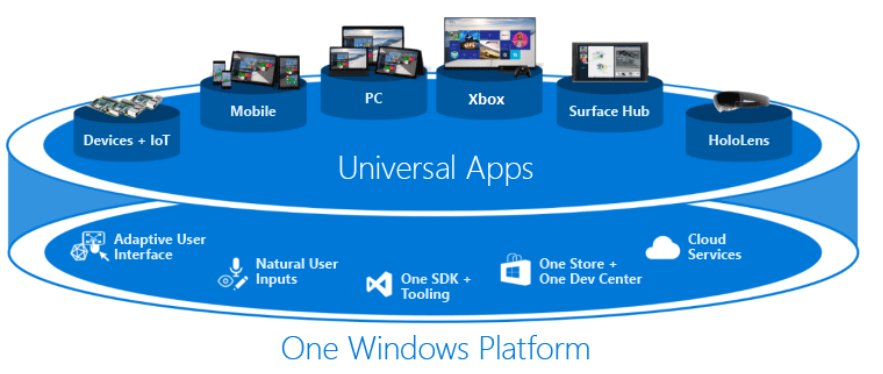
\includegraphics[width=0.7\linewidth]{images/screenshot001}
	\caption{Darstellung der UWP}
	\label{fig:screenshot001}
\end{figure}

Dennoch kann für jedes Gerät spezieller Code geschrieben werden sodass die Anwendung ein unterschiedliche Verhalten je nach Gerät aufweist. Außerdem bietet UWP universelle Steuerelemente, womit eine Benutzeroberfläche entwickelt werden kann, welche sich an die Auflösung, DPI-Dichte, Eingabeart von Geräten anpasst.
\\\\
UWP ermöglicht das Entwickeln mittels Visual C++, C\#, Visual Basic und JavaScript, wobei mit den Programmiersprachen Visual C++, C\# und Visual Basic XAML verwendet werden kann um die Benutzeroberfläche zu definieren. \cite{UWPAllgemein}
\\\\
XAML beschreiben
\\\\
Bei dieser Übung wurde C\# mit XAML zur Umsetzung der Aufgabe verwendet.

\subsection{Visual Studio}

Als am besten geeignetes Tool erweist sich Visual Studio, welches eine optimale Unterstützung für die Entwicklung von UWP Apps bietet. Bei dieser Übung wurde Visual Studio 2017 Enterprise Edition verwendet, wobei darauf zu achten ist, dass zur Verwendung von Emulatoren für andere Geräte, wie zum Beispiel Smartphones, HoloLens, ... , Visual Studio 2015 installiert sein muss. Zwar können die Emulatoren für Visual Studio 2017 gedownloadet werden, diese werden aber im Editor dann nicht angezeigt, wenn Visual Studio 2015 nicht installiert ist.
\\\\
Im Visual Studio Installer kann im Reiter "Einzelne Komponenten" Emulatoren für die gewünschte Windows 10 Version gedownloadet werden.

\begin{figure}
	\centering
	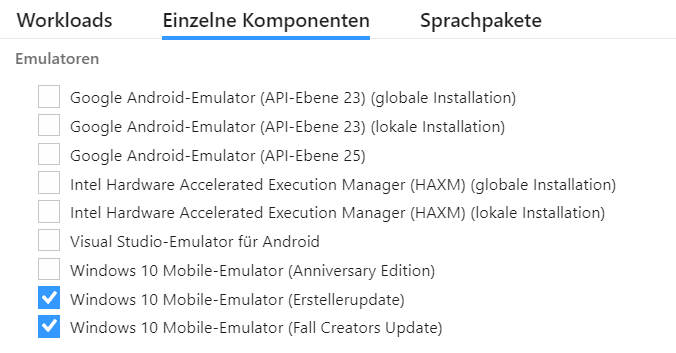
\includegraphics[width=0.7\linewidth]{images/screenshot002}
	\caption{Installieren von Emulatoren}
	\label{fig:screenshot002}
\end{figure}

In Visual Studio kann anschließend die App auf den gewünschten Gerät ausgeführt werden.

\section{REST - Schnittstelle}

Als REST - Schnittstelle wurde die entwickelte Anwendung für die Übung GK9.3 verwendet. Diese wurde nur leicht angepasst, sodass JSON Objekte gesendet werden.

\subsection{Deployen}

Die Anwendung ist im Unterverzeichnis "Cloud-Datenmanagement-Json" zu finden. Diese kann einfach deployed werden, da es sich um ein mit Maven erstelltes Programm handelt.
\\\\
Mittels folgendem Befehl wird die Anwendung auf den Port 8080 lokal gestartet.

\begin{code}{bash}
	mvn tomcat7:run-war
\end{code}

\subsection{Verwendung}

Die REST-Schnittstelle bietet 3 Funktionen, das Anmelden eines neuen Benutzers, den Login mit einem bestehenden Account und das Löschen eines Benutzerkontos.

\subsubsection{Registrierung}

Bei der Registrierung muss der Vorname, der Nachname, die E-Mail-Adresse, ein Passwort sowie eine Passwort Wiederholung eingegeben werden. Diese Eingaben werden als Parameter an die Schnittstelle gesendet, nachfolgend ist ein Beispielaufruf zu sehen:

\begin{code}{bash}
	Inhalt...
\end{code}

\section{Mobilen Applikationen}

\subsection{UML}

\subsection{Register}

\subsection{Login}

\subsection{Mainpage}

\subsection{Deployen}

\section{Testen}

\subsection{UI Automation}

\subsection{Testaufbau}




\clearpage

\section{Konfiguration}
\subsection{Optionen}
\begin{tabularx}{\textwidth}{l X}
{\small \verb|landscape|}    & Richte das Dokument vertikal aus.\\
{\small \verb|minted|}       & Nutze das \texttt{minted} Paket zur Quelltextdarstellung.\\
{\small \verb|natbib|}       & Nutze NatBib zur Literaturverwaltung.\\
{\small \verb|nobib|}        & Deaktiviere die Literaturverwaltung.\\
{\small \verb|nofonts|}      & Nutze die Standard \LaTeX ~Schriftarten.\\
{\small \verb|noglo|}        & Deaktiviere Akronyme und das Glossar.\\
{\small \verb|nologos|}      & Zeichne keine Logos auf der Titelseite.\\
{\small \verb|notitle|}      & Zeichne keine Titelseite.\\
{\small \verb|notoc|}        & Zeichne kein Inhaltsverzeichnis.\\
{\small \verb|notable|}      & Zeichne keine Tabelle auf der Titelseite.
\end{tabularx}

\subsection{Variablen}
Variablen werden über Kommandos gesetzt, die als Parameter den gewünschten Wert erhalten.
\begin{code}{tex}
\myvariable{value}
\end{code}

\begin{tabular}{l l}
\textbf{Kommando} & \textbf{Inhalt}\\

{\small \verb|mysubtitle|} 	& Untertitel oder Zugehörigkeit\\
{\small \verb|mysubject|} 	& Thema / Fach, welches bearbeitet wird\\
{\small \verb|mycourse|} 	& Kurs / Klasse welche(r) besucht wird\\
{\small \verb|myteacher|} 	& Betreuende Lehrkraft\\
{\small \verb|myversion|} 	& Aktuelle Version des Dokuments\\
{\small \verb|mybegin|} 	& Datum des Beginns\\
{\small \verb|myfinish|} 	& Datum an dem die Arbeit beendet wurde
\end{tabular}

\newpage
\section{Kommandos}\label{sec:Kommandos}
\subsection{\texttt makefig}

\begin{listing}
\begin{code}{tex}
\makefig{images/hit-logo.png}{height=2cm}{
    Mit Beschreibung und Label  % (Optional)
}{
    fig:caption-label           % (Optional)
}
\end{code}
\caption{\texttt makefig}
\label{lst:makefig}
\end{listing}
\makefig{images/hit-logo.png}{height=2cm}{Mit Beschreibung und Label}{fig:caption-label}

\subsection{\texttt vardef}
\begin{listing}
\begin{code}{tex}
$$e^{i*\pi} = -1$$
\end{code}

$$e^{i*\pi} = -1$$

\begin{code}[firstnumber=last]{tex}
\begin{vardef}
    \addvardef{$e$}{Eulersche Zahl}
    \addvardef{$\pi$}{Kreiszahl}
    \addvardef{$i$}{Imagin\"are Einheit}
\end{vardef}
\end{code}

\begin{vardef}
    \addvardef{$e$}{Eulersche Zahl}
    \addvardef{$\pi$}{Kreiszahl}
    \addvardef{$i$}{Imaginäre Einheit}
\end{vardef}

\caption{\texttt vardef}
\label{lst:vardef}
\end{listing}

\newpage
\section{Anwendung}\label{sec:Anwendung}
Hier sollen die Schritte der Laborübung erläutert werden. Hier sind alle Fragestellungen der Lehrkraft zu beantworten. Etwaige Probleme bzw. Schwierigkeiten sollten ebenfalls hier angeführt werden.

In diesem Fall werden einige \LaTeX-Elemente dokumentiert, welche bei der Kreation von Protokollen behilflich sein könnten.

\subsection{Tabellen}
\begin{table}[H]
	\center
	\begin{tabular}{| c | l |}
		\hline Header 	& Kopf\\ \hline\hline
		\textbf{Lorem} 	& Ipsum dolor sit amet, consetetur sadipscing elitr\\ \hline
		\textbf{Ipsum} 	& At vero eos et accusam et justo duo dolores et ea rebum.\\
						& Stet clita kasd gubergren, no sea takimata sanctus\\ \hline
		\textbf{Dolor} 	& Consetetur sadipscing elitr, sed diam nonumy\\\hline
	\end{tabular}
	\caption{Tabular}
	\label{tab:tabular}
\end{table}

\subsubsection{TabularX}
TabularX erlaubt die Angabe der Größe der Tabelle und bietet zudem den Reihentyp \texttt{X}, der die verbleibende Größe neben anderen Reihen mit anderen \texttt{X} Reihen teilt.
\\\\
ACHTUNG: Die Verwendung von \verb|\codein|, \verb|\mintinline| oder \verb|\lstinline| ist in einer TabularX Umgebung nicht möglich!
\begin{table}
    \center
    \begin{tabularx}{\textwidth}{| c | X |}
        \hline Header 	& Kopf\\ \hline\hline
        \textbf{Lorem} 	& Ipsum dolor sit amet, consetetur sadipscing elitr\\ \hline
        \textbf{Ipsum} 	& At vero eos et accusam et justo duo dolores et ea rebum.\\
            			& Stet clita kasd gubergren, no sea takimata sanctus\\ \hline
        \textbf{Dolor} 	& Consetetur sadipscing elitr, sed diam nonumy\\\hline
    \end{tabularx}
    \caption{TabularX}
    \label{tab:tabularx}
\end{table}

\newpage
\subsection{Aufzählung}
\begin{itemize}
	\item Element einer Aufzählung
	\begin{itemize}
        \item Erstes eingerücktes Element einer Aufzählung
        \item Zweites eingerücktes Element einer Aufzählung
    \end{itemize}
\end{itemize}

\subsubsection{Outlines}
\begin{outline}
    \1 Element einer Aufzählung
        \2 Erstes eingerücktes Element einer Aufzählung
        \2 Zweites eingerücktes Element einer Aufzählung
\end{outline}

\subsection{Glossar}
Zur Verwaltung des Glossars wird standardmäßig die Datei \texttt{glossaries.tex} verwendet, wobei sowohl Definitionen als auch Akronyme definiert werden können.
\\\\
Als Beispiel wurde ein Akronym für \gls{ac-syt} und eine Definition zu \gls{ac-syt} selbst hinzugefügt.

\inputcode{tex}{glossaries.tex}

Im Dokument selbst kann ein Akronym mittels \verb|\gls{ac-syt}| verwendet werden. Beachte, dass ein Akronym welches bereits im Dokument verwendet wurde, bei der ersten Verwendung ausgeschrieben und danach immer gekürzt wird.
\\\\
Mit \verb|\gls{syt}| kann zum Beispiel eine Referenz zur Definition von \gls{syt} hinzugefügt werden.

\subsection{Zitate}
Zitate sollten gesammelt in der Datei \texttt{bib.bib} verwaltet werden.

\newpage
\subsection{Quelltext}
\begin{listing}
\ifminted   \codeline{tex}{\begin{code}[]{java}}
\else       \codeline{tex}{\\begin\{code\}[]\{java\}}\fi
\begin{code}[firstnumber=last]{java}
// Ich bin ein Kommantar!
public static void main(String[] args) {
    System.out.println("Ich bin ein Array!")
}
\end{code}
\ifminted   \codeline[firstnumber=last]{tex}{\end{code}}
\else       \codeline[firstnumber=last]{tex}{\\end\{code\}}\fi

\caption{Java Code}
\label{lst:java-code}
\end{listing}
~\\
Die Darstellung von Quelltext im Text ist über das Kommando \verb|\codein[options]{lang}{code}| möglich.
\\\\
Eine einzelne Zeile kann mittels
\ifminted   \codeline{tex}{\codeline[options]{lang}{code}}
\else       \codeline{tex}{\\codeline[options]\{lang\}\{code\}}\fi
eingefügt werden.

\subsubsection{Listings}
\begin{listing}
\ifminted   \codeline{tex}{\begin{lstlisting}[language=Java, caption=Java Lstlisting]}
\else       \codeline{tex}{\\begin\{lstlisting\}[language=Java, caption=Java Lstlisting]}\fi
\begin{code}[firstnumber=last]{java}
// Ich bin ein Kommantar!
public static void main(String[] args) {
    System.out.println("Ich bin ein Array!")
}
\end{code}
\ifminted   \codeline[firstnumber=last]{tex}{\end{lstlisting}}
\else       \codeline[firstnumber=last]{tex}{\\end\{lstlisting\}}\fi
\caption{Java Lstlisting}
\label{lst:java-lstlisting}
\end{listing}

\newpage
\subsubsection{Minted}
Benötigt die Option \texttt{minted}.
\paragraph{Umgebung}~\\
\begin{listing}
\ifminted   \codeline{tex}{\begin{minted}[options]{java}}
\else       \codeline{tex}{\\begin\{minted\}[]\{java\}}\fi
\begin{code}[firstnumber=last]{java}
// Ich bin ein Kommantar!
public static void main(String[] args) {
    System.out.println("Ich bin ein Array!")
}
\end{code}
\ifminted   \codeline[firstnumber=last]{tex}{\end{minted}}
\else       \codeline[firstnumber=last]{tex}{\\end\{minted\}}\fi
\caption{Minted Umgebung}
\label{lst:minted-env}
\end{listing}

\paragraph{Zeile}~\\
\begin{listing}
\begin{code}{tex}
\mint[options]{lang}|code|
\end{code}
\caption{Minted Einzeiler}
\label{lst:minted-line}
\end{listing}

\begin{listing}
\begin{code}{tex}
\mintinline[options]{lang}{code}
\end{code}
\caption{Minted Inline}
\label{lst:minted-inline}
\end{listing}